%%% Для сборки выполнить 2 раза команду: pdflatex <имя файла>

\documentclass[a4paper,12pt]{article}

\usepackage[margin=1in]{geometry}
\usepackage{ucs}
\usepackage[utf8x]{inputenc}
\usepackage[english, russian]{babel}
%\usepackage{cmlgc}
\usepackage{graphicx}
\usepackage{listings}
\usepackage{xcolor}
\usepackage{wrapfig}
\usepackage{sidecap}
%\usepackage{courier}

\makeatletter
\renewcommand\@biblabel[1]{#1.}
\makeatother

\newcommand{\myrule}[1]{\rule{#1}{0.4pt}}
\newcommand{\sign}[2][~]{{\small\myrule{#2}\\[-0.7em]\makebox[#2]{\it #1}}}

% Поля
\usepackage[top=20mm, left=30mm, right=10mm, bottom=20mm, nohead]{geometry}
\usepackage{indentfirst}

% Межстрочный интервал
\renewcommand{\baselinestretch}{1.50}

% Согласно ГОСТу в заголовках таблиц, листинго кода, рисунков
% в качестве разделителя номера и текста заголовка используется тире 
\usepackage[labelsep=endash]{caption} 
\captionsetup[table]{skip=1ex}

% Размер полосы разделителя между столбцами таблицы по умолчанию
\setlength{\tabcolsep}{1em}

% Формат листинга по умолчанию
\lstdefinestyle{mylisting}{%
    basicstyle=\ttfamily,
    columns=fullflexible,
    keepspaces=true,
    commentstyle=\normalshape,
    keywordstyle=\bfseries,
    showstringspaces=false,
    captionpos=t,
    belowcaptionskip=1.5ex,
    frame=lines
}

\begin{document}

%%%%%%%%%%%%%%%%%%%%%%%%%%%%%%%
%%%                         %%%
%%% Начало титульного листа %%%

\thispagestyle{empty}
\begin{center}


\renewcommand{\baselinestretch}{1}
{\large
{\sc Петрозаводский государственный университет\\
Институт математики и информационных технологий\\
	Кафедра Информатики и математического обеспечения
}
}

\end{center}


\begin{center} 
Направление подготовки бакалавриата \\
09.03.04 Программная инженерия \\
Профиль направления подготовки бакалавриата \\
``Системное и прикладное программное обеспечение''

\end{center}

\vfill

\begin{center}
{\normalsize Курсовая работа по теме:} \\
\medskip

%%% Название работы %%%
	{\Large \sc {Разработка 2D Roguelike игры на движке Unity}} \\
\end{center}

\medskip

\begin{flushright}
\parbox{11cm}{%
\renewcommand{\baselinestretch}{1.2}
\normalsize
	Выполнил\\
%%% ФИО студента %%%
студент группы 22207:
\begin{flushright}
	И. Е. Мельников \sign[подпись]{4cm}
\end{flushright}
%%%%%%%%%%%%%%%%%%%%%%%%%
% девушкам применять "Выполнила" и "студентка"
%%%%%%%%%%%%%%%%%%%%%%%%%






Научный руководитель\\ к.т.н., доцент кафедры ИМО:\\
%%% степень, звание ФИО научного руководителя %%%
%%% Первый руководитель 
%%% {автор задачи, если выбран мини проект} 
\begin{flushright}
{ C. А. Марченков \sign[подпись]{4cm} }
\end{flushright}


Итоговая оценка
\begin{flushright}
  \sign[оценка]{4cm}
\end{flushright}
}
\end{flushright}

\vfill

\begin{center}
\large
    Петрозаводск --- 2022
\end{center}

%%% Конец титульного листа  %%%
%%%                         %%%
%%%%%%%%%%%%%%%%%%%%%%%%%%%%%%%

%%%%%%%%%%%%%%%%%%%%%%%%%%%%%%%%
%%%                          %%%
%%% Текст отчета             %%%


\newpage
\tableofcontents

\newpage
\section*{Введение}
\addcontentsline{toc}{section}{Введение}
\large {
Мой выбор пал на игру жанра Roguelike. Что это за жанр? Принято считать, что характерными особенностями классического roguelike являются генерируемые случайным образом уровни, пошаговость и необратимость смерти персонажа, то есть в случае его гибели игрок не может загрузить игру и должен начать её заново.

Затем необходимо опеделиться с движком. Unity — это игровой движок, на котором разрабатывают мобильные игры и проекты для ПК и консолей. Это удобный бесплатный инструмент для начинающих разработчиков, в нем можно создавать проекты в одиночку. На этом движке созданы такие популярные проекты как Genshin Impact, Hearthstone, Outlast, Cuphead, Pokemon GO и другие... И не без причины, ведь Unity обладает рядом примуществ, такими как:
\begin{itemize}
    \item Доступность. Начать разработку и выпускать свои первые проекты можно бесплатно.
    \item Низкий порог вхождения в разработку. Некоторые игры получится собрать, даже если вы не умеете писать код.
    \item Обучение. Для новичков создали подробные бесплатные обучающие материалы.
    \item Поддержка сообщества. Комьюнити Unity-разработчиков большое, поэтому велика вероятность, что с возникшей проблемойс кто-то уже сталкивался и готов помочь.
\end{itemize}

Рассматривая огромное кол-во других 2D игр, было решено реализовать графику в стиле Pixel-Art. С ней легко работать, можно использовать почти любой графический редактор. Да и сами спрайты при хорошем исполнении выглядят довольно атмосферно и всегда мне симпатизировали.
} \\ 
 \\


\textbf{Цели:}
\begin{itemize}
    \item Приобрести навыки и опыт работы с движком Unity
    \item Повысить свою квалификацию по ходу работы с C\# и системой Tilemap для Unity
    \item Закрепить имеющиеся навыки во время работы с:
    \begin{itemize}
     \item Языками разметки: LaTeX, Beamer, HTML
    \item Языком программирования: C\#
    \item Веб-сервисом для хостинга: GitHub
    \end{itemize}
\end{itemize}

\textbf{Задачи:} 
\begin{itemize}
    \item Освоиться с интерфейсом Unity
    \item Создание Roguelike игры
    \item Сборка готового билда для скачивания другими пользователями
    \item Добавление контента в игру
    \item Проанализировать полученные результаты и сформулировать выводы, что удалось реализовать, что неудалось, какой получили опыт в результате работы
    \item Создание документации
\end{itemize}

\newpage
\section{Реализация}

\subsection{Создание проекта }

Запускаем движок и на странице проектов выбираем "Новый" \\
Задаем необходимые параметры, а именно: название проекта, шаблон графики, расположение на диске. Также есть возможность включить аналитику от Unity, чтобы позволить им собирать данные вашего проекта и предоставлять Вам аналитику схожих проектов.\\
После загрузки проекта появляется возможность настроить под себя планировку элементов движка и приступить к работе \\
\\
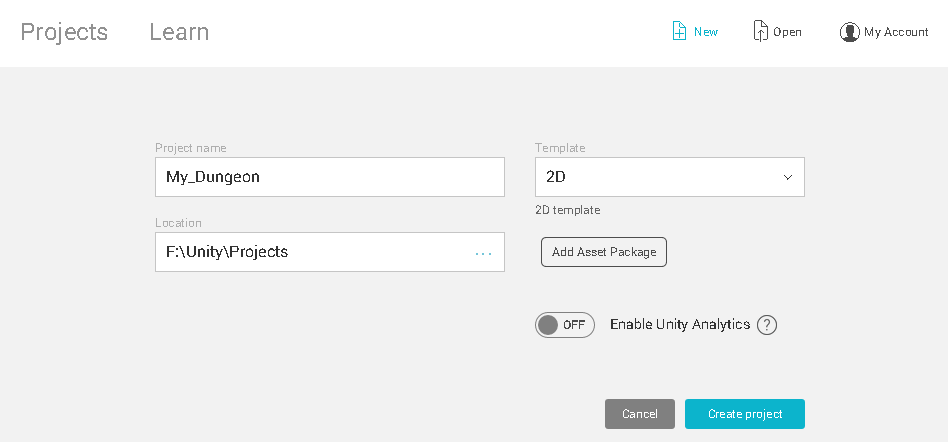
\includegraphics[width = 400px, height=220px]{pictures/project.png}

\newpage
\subsection{Подготовка к созданию игры}
Начать стоит с необходимых разделов \\
\begin{itemize}
    \item 1. В окне проекта создаем папку Artwork. И внутри нее создаем папки Animations и Artwork. Здесь будет находиться все необходимое, что касается аниматоров, анимаций, Tile'ы для Tilemap'ов наших уровней, атласыв и шрифты.
    \item 2. Папка Prefab будет хранить готовые игровые объекты, которые надо будет использовать больше одного раза, чтобы не создавать их заново.
    \item 3. Папка Scenes будет хранить уровни игры, или же сцены, со всеми размещенными на ней объектами.
    \item 4. Папка Scripts будет хранить написанные на C\# скрипты для игровых объектов
    \item 5. После этого создаем главную сцену, которая послужит Intro-уровнем игры
    \end{itemize}
\noindent


\centerline{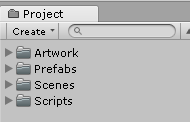
\includegraphics[width = 450px]{pictures/folders.png}} \\
\vspace{2mm}
\centerline{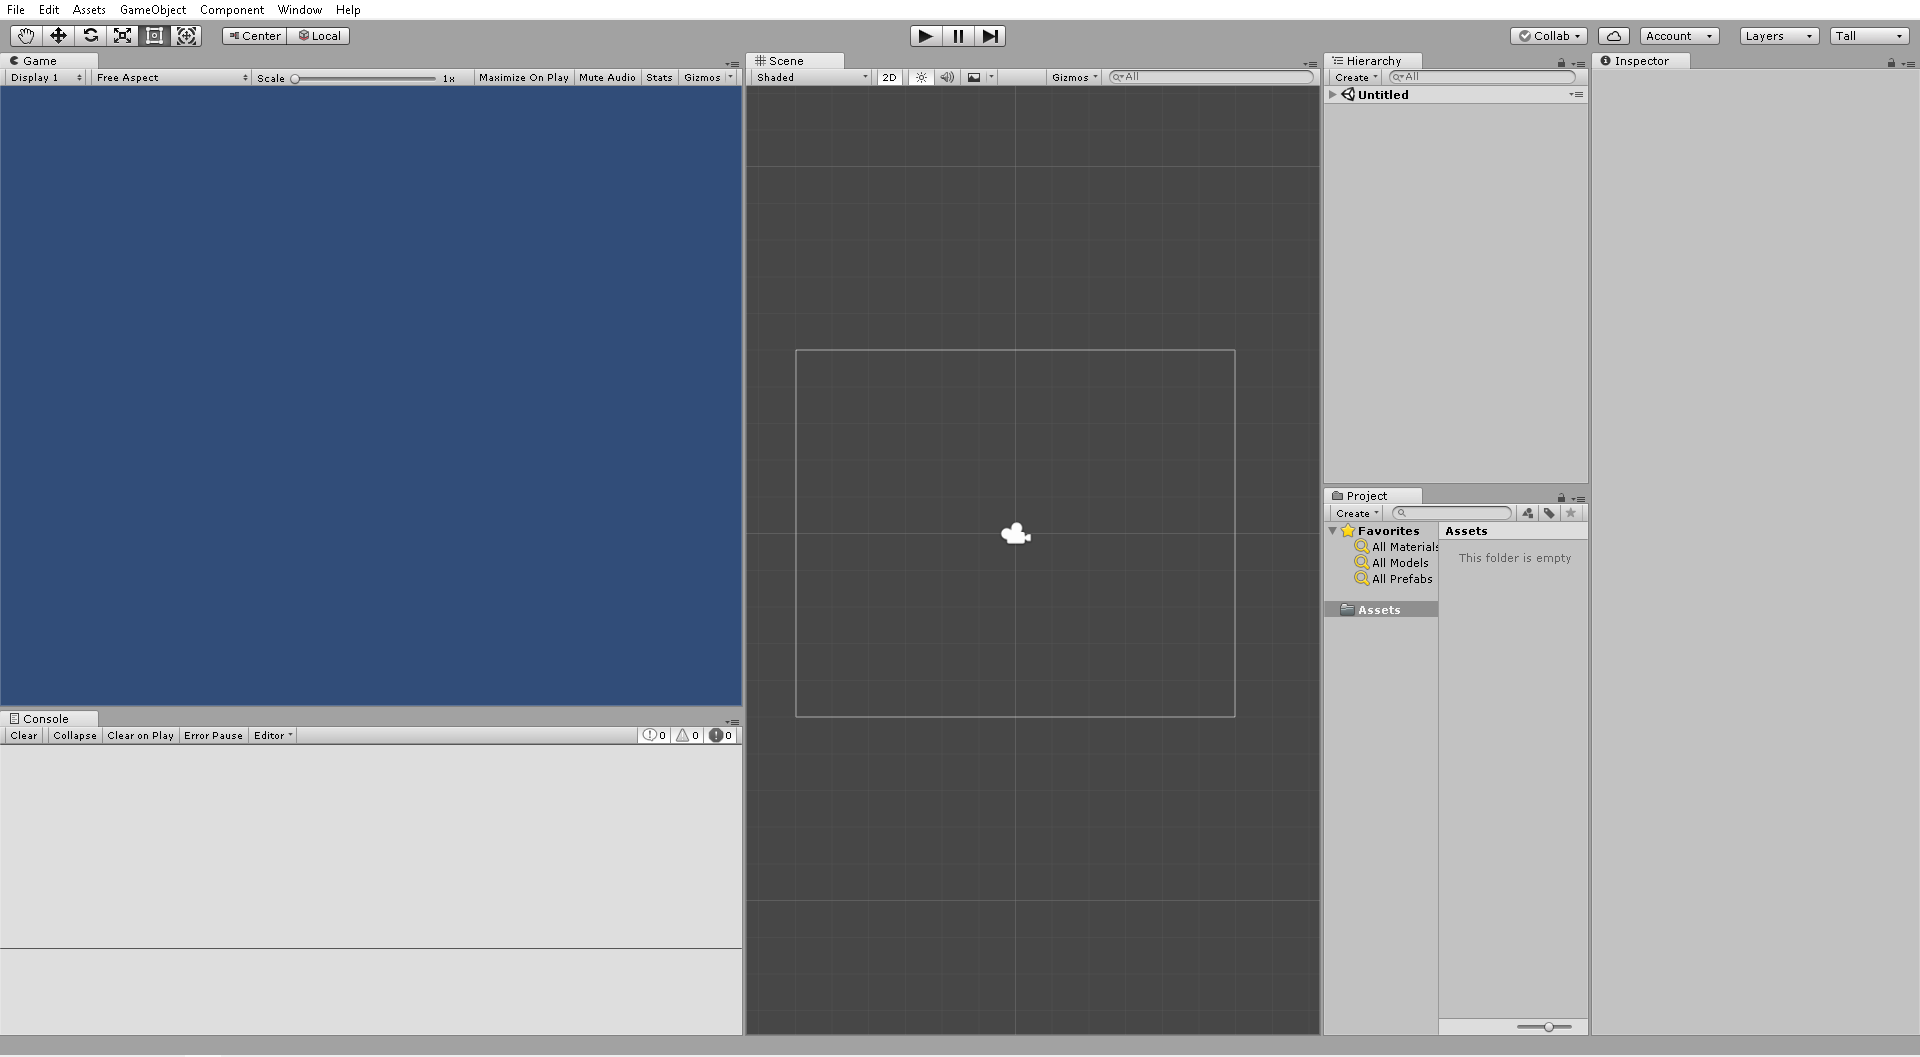
\includegraphics[width = 450px]{pictures/layout.png}}

\newpage
\subsection{Выбор спрайтов}
\noindent
Ввиду своих слабых творческих способностей было принято решение использовать готовый сет спрайтов, бесплатный, в том числе и для коммерческих проектов.\\ 
Сет представляет из себя набор около 300 различных спрайтов различных моделей оружий, персонажей, монстров, стен, сундуков и всего другого необходимого для жанра Roguelike \\
После загрузки атласа вырезаем из него первые спрайты, а именно, игровых персонажей. \\
Что удобно в данном наборе спрайтов, так это то, что большинство необходимых спрайтов умещается в размеры 16 на 16 пикселей, что позволяет иметь некий стандартизированный их размер. \\
\noindent
\centerline{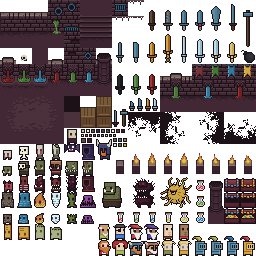
\includegraphics[width = 400px]{pictures/Atlas.png}}


\newpage
\begin{center}
\textbf{Написание кода}\\
\end{center}
После добавления первых объектов можно приступать к написания первых скриптов \\
Начнем с добавления компонента главному герою, а именно скрипта Player \\

\centerline{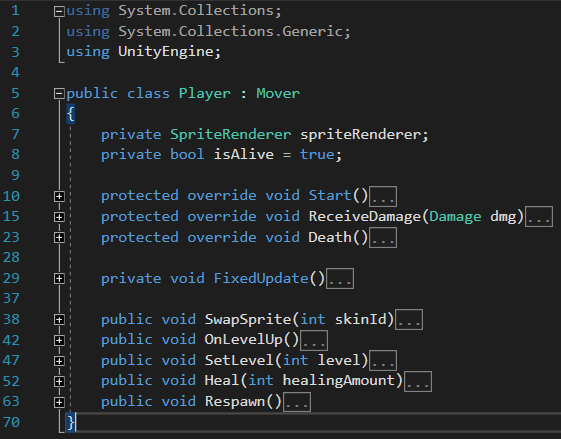
\includegraphics[width = 300px, height=300px]{pictures/player1.png}}

По началу в Player.cs будет находится все, что связано с движением объекта. Обработка координат и векторов будет происходить в функции FixedUpdate. Также создается Box Collider. Он отвечает за область объекта которая будет сталкиваться с другими, тоже имеющими такую область. \\ 
\centerline{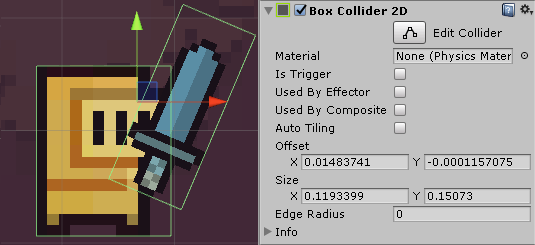
\includegraphics[width = 450px, height=300px]{pictures/boxcoll.png}}

Создадим скрипт CameraMotor.cs для движения камеры и реализуем в нем функцию LateUpdate. Скрипт будет указывать камере, какой объект необходимо отслеживать, а также границы, в которых этот объект будет отслеживаться. \\
После этого можно отвлечься и заняться прорисовкой уровня, чтобы персонаж не ходил по пустоте. Для этого переносим все необходимые спрайты в палитру, и заполняем ими созданные Tilemap'ы. Слоев должно быть несколько, чтобы можно было отрисовывать более детальные объекты с помощью накладывания одного на другой. Одним из слоев будет слой, блокирующий игроку доступ в определенные области. Для этого добавляем Tilemap Collider, отвечающий за столкновение и снимаем галочку с рендера данного слоя в игре. \\
Сразу создаем новую сцену - следующий уровень для игрока, и отрисовываем и ее. \\
\centerline{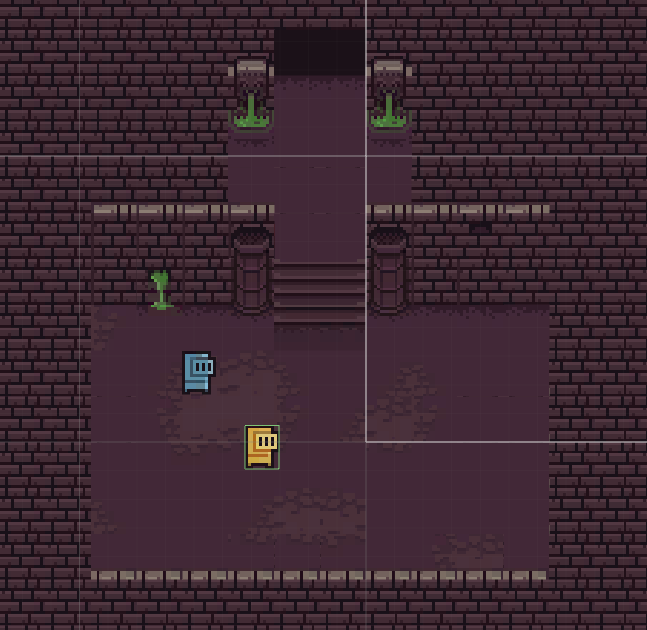
\includegraphics[width = 300px, height=300px]{pictures/level1.png}} \\
\vspace{2mm}
\centerline{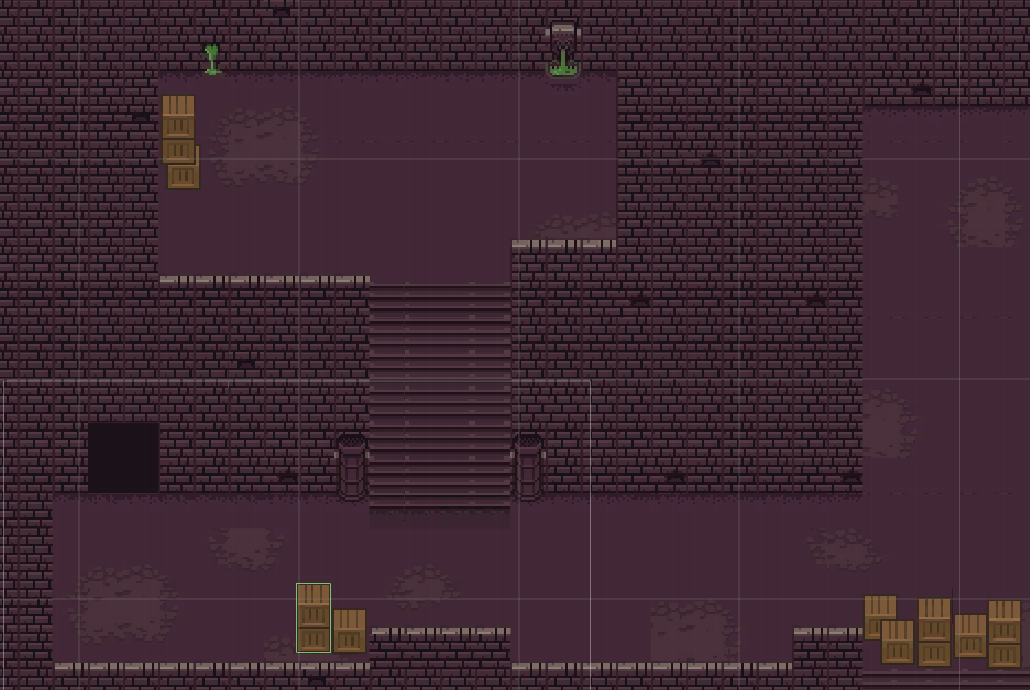
\includegraphics[width = 400px, height=300px]{pictures/level2.png}}

Пропишем скрипт для объектов, с которыми игрок сможет взаимодействоать на отрисованной карте. В Collidable.cs реализована функция Update, которая будет отслеживать с какими именно объектами в данный момент "сталкивается" игрок. \\
Сундуки должны награждать игрока золотом. Но кроме него в игре могут присутствовать другие объекты для собирания, для этого создадим класс Collectable.cs, который будет наследовать класс Collidable.cs, и пропишем в нем логику собирания. \\
\centerline{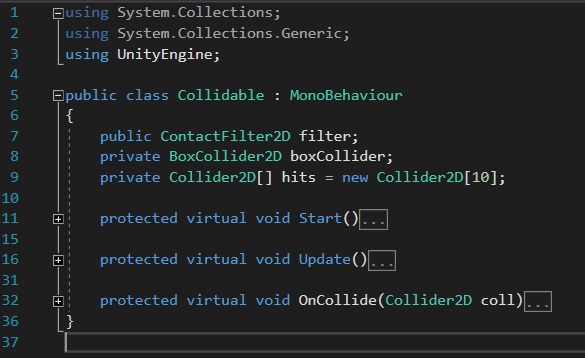
\includegraphics[width = 300px, height=200px]{pictures/coll.png}}
\centerline{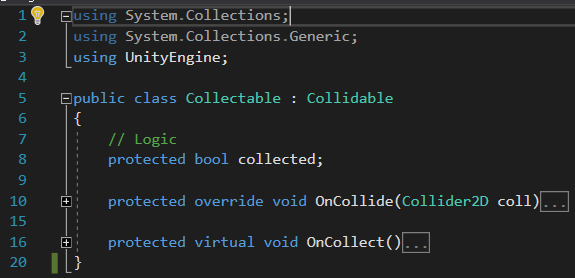
\includegraphics[width = 300px, height=200px]{pictures/coll1.png}}

Теперь для сундуков напишем отдельный скрипт Chest.cs, который будет наследовать класс Collectable и пропишем в нем смену состояние сундука и его спрайта. \\
Для портала переноса на следующий уровень создадим следующий скрипт Portal.cs. Он наследует класс Collidable, проверяет что в портале находится игрок, и только тогда загружает следующую сцену. \\
\centerline{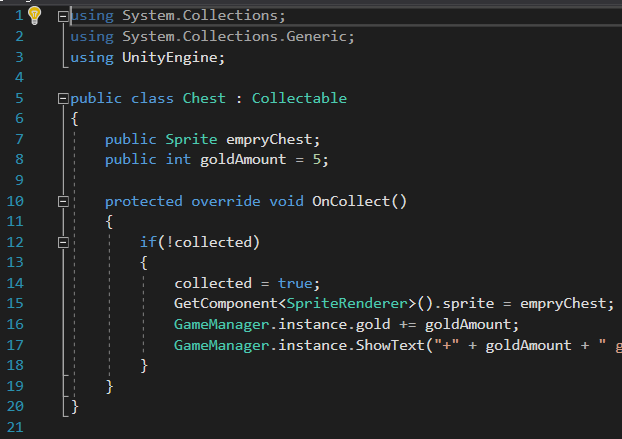
\includegraphics[width = 300px, height=200px]{pictures/chest.png}} \\
\centerline{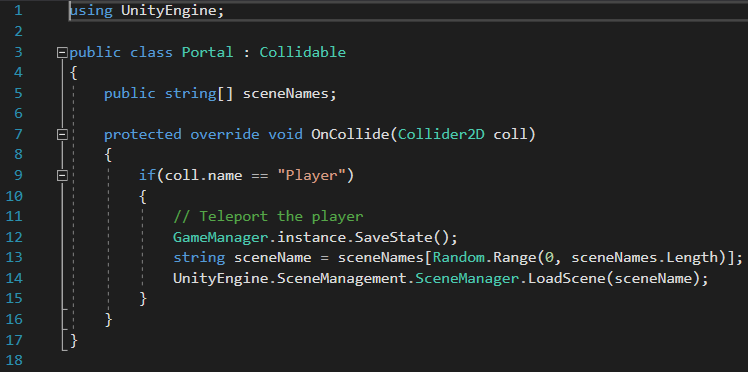
\includegraphics[width = 300px, height=200px]{pictures/portal.png}}

После этого создадим GameManager в котором будет находиться большинство варьирующихся переменных и ресурсов, таких как спрайты героев, оружий, цены на оружие, опыт, кол-во золота, кол-во жизней и др. А также референсы на скрипт для игрока, скрипт для оружия и другие будующие скрипты. \\
Также пропишем в нем состояние сохранения и состояние загрузки, где в и из string переменной будут грузиться некоторые данные об игроке (золото, опыт, уровень оружия) \\
\centerline{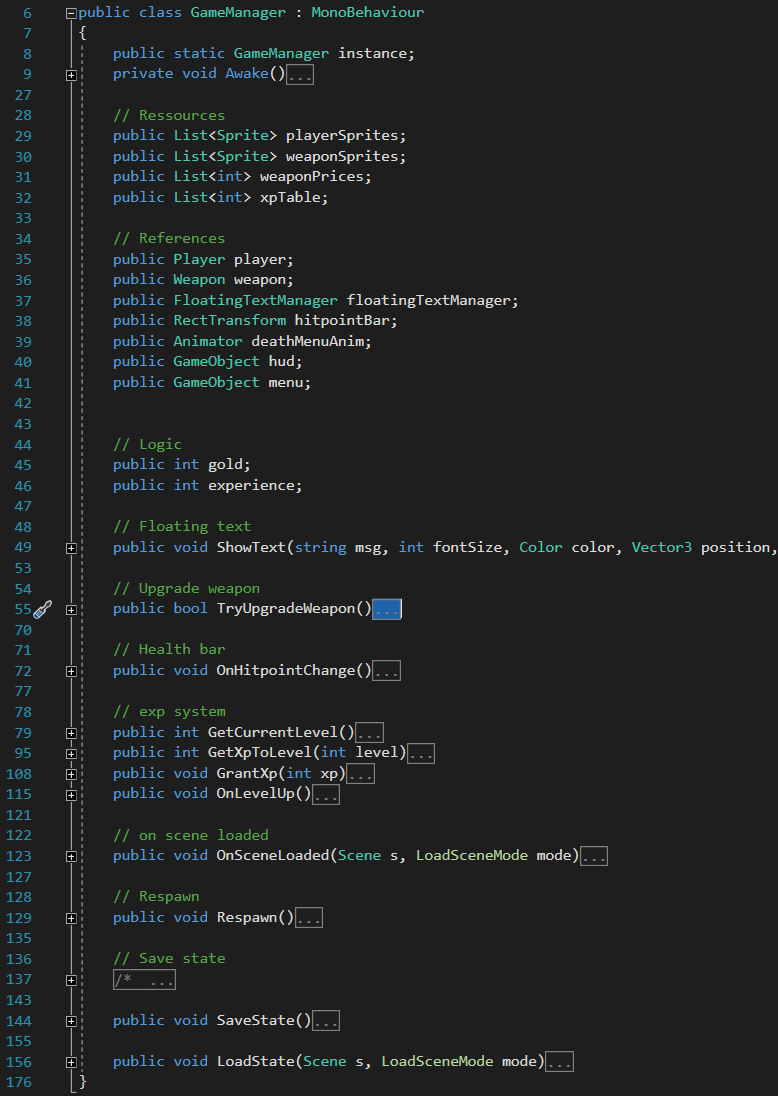
\includegraphics[width = 250px, height=300px]{pictures/gm.png}}

Также пропишем скрипт FloatingText.cs для всего всплывающего текста. В нем будут функции Show и Hide, а также функция отрисовки сообщения в кадре в зависимости от времени. \\
Необходим также менеджер всплывающих сообщений FloatingTextManager.cs, чтобы реиспользовать один и тот же объект для отображения различных сообщений, каждый раз заменяя размер шрифта, цвет и т.д. В Show пропишем также длительность и положение сообщения относительно камеры. \\
В GameManager'е также пропишем функцию для вызова менеджера текста.\\
После этого можно начать вызывать функию в Chest.cs для вызова сообщения о награждении золотом. \\
\centerline{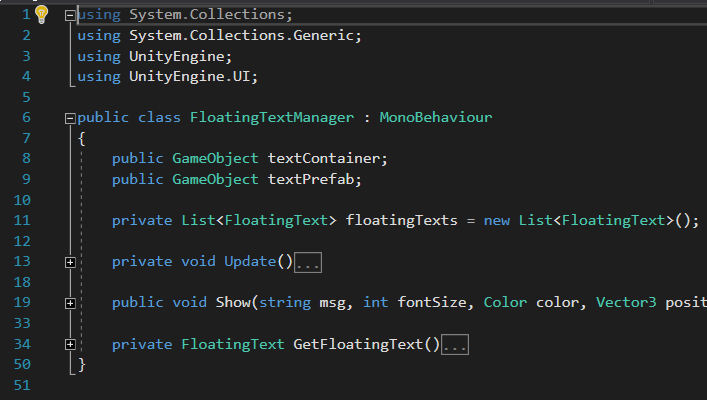
\includegraphics[width = 300px, height=200px]{pictures/fm.png}}

\newpage
\subsection{Боевая система}
Перейдем к боевой системе.\\
Переносим оружие на сцену и добавляем ему Box Collider'а и создаем скрипт Weapon.cs. В нем будут храниться массивы с уроном и отдачей по противнику, переменные уровня оружия, кулдауна удара и другие переменные для функционирования боевой системы. Скрипт будет следить за оружием в реальном времени: его кулдауном, хитбоксом и уровнем. \\
В скрипте также будет находится вызов структуры для нанесения урона, и это новый скрипт Damage.cs. Он будет служить контейнером для урона по объекту, на который мы будем его отправлять. \\

Теперь создадим скрипт Fighter.cs, который будет наследоваться нашим игроком и врагами. Он будет наделять их здоровьем и функцией для получения урона. \\
В связи с этим создадим скрипт Enemy.cs, наследующий класс Fighter, содержащий все данные о враге (здоровье, опыт, хитбокс удара и урона, состояние преследования и другое) \\
Чтобы вооружить врага создадим скрипт EnemyHitbox, наследующий класс Collidable, где будем отправлять урон по игроку, если объекты сталкиваются.

Самое время создать скрипт движения Mover.cs, наследующий класс Fighter. Сюда перейдет большая часть скрипта Player.cs, т.к. теперь Mover будет отвечать за передвижение объекта, а Player.cs в свою очередь теперь будет наследовать класс Mover. Скрипт будет работать с векторами, следить за напрвлением движения, толчков и заставлять объект двигаться.\\
\centerline{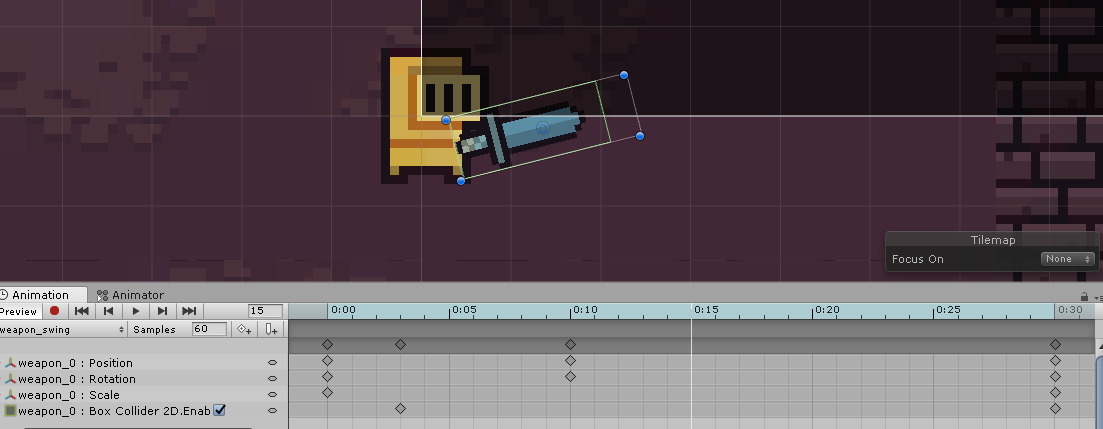
\includegraphics[width = 400px, height=200px]{pictures/anim.png}} \\
\centerline{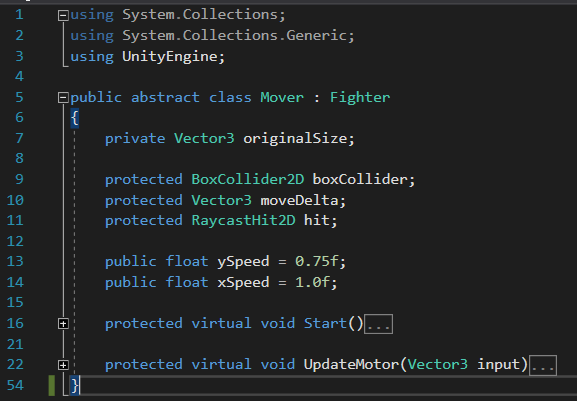
\includegraphics[width = 300px, height=200px]{pictures/mover.png}} 

\newpage
\subsection{Анимация}
Создание анимации в Unity происходит довольно просто. \\
Для начала нужно добавить объекту компонент Animator. \\
После чего в окне анимации, создаем клип и переходим непосредственно к анимации. \\
На концах временной шкалы задаем состояние нашего объекта, и Animator самостоятельно заполнит пространство. Единственное с чем придется повозиться, это с хитбоксом, который должен активироваться и деактивироваться на определенной секунде.\\

Далее в аниматоре соединяем состояния согласно логике анимации и привязываем переходы к триггерам. И все, что остается, это добавить триггеры в код. Для этого в функции удара выполняем вызов необходимого триггера. \\
\centerline{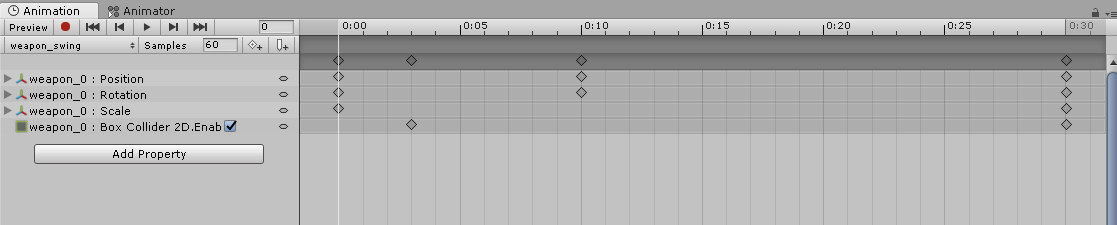
\includegraphics[width = 400px, height=80px]{pictures/anim1.png}} \\
\centerline{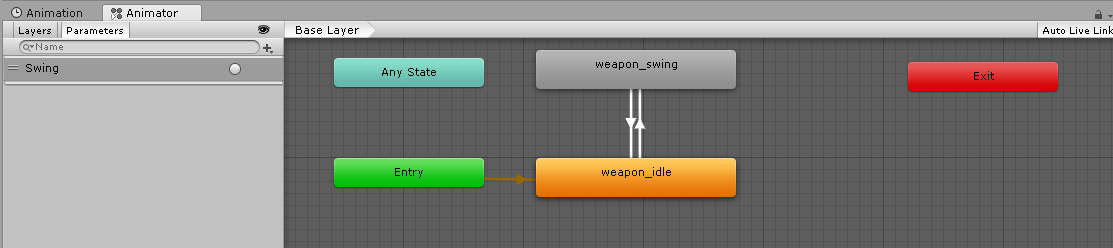
\includegraphics[width = 400px, height=80px]{pictures/anim2.png}}

\newpage
\subsection{Меню}
Для вызова меню понадобиться канвас с самим меню \\
\centerline{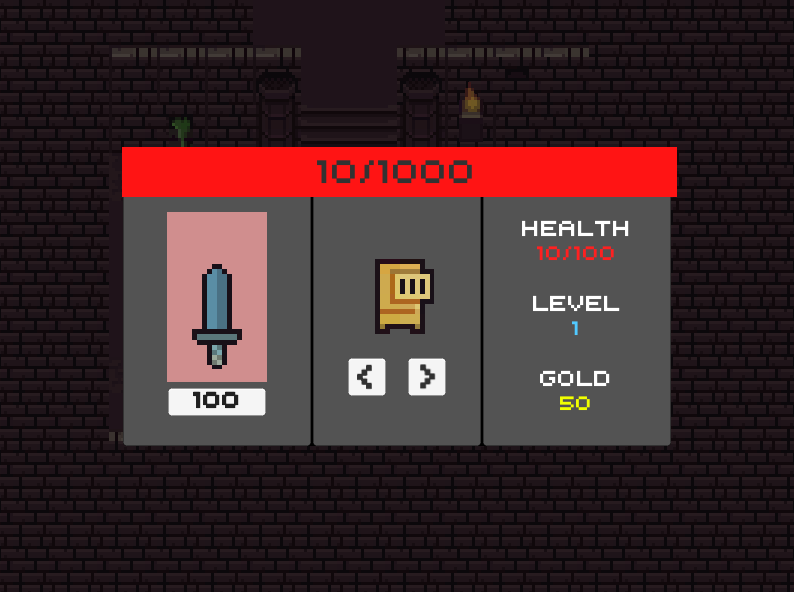
\includegraphics[width = 380px, height=280px]{pictures/menu.png}}

и канвас интерфейса с кнопкой. \\
\centerline{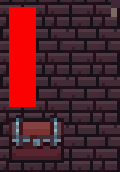
\includegraphics[width =50px, height=80px]{pictures/hud.png}}

Создаем анимацию появления меню по уже известному принципу. Триггерами анимации послужат кнопки в интерфейсе, для которых в Unity уже написан готовый скрипт. Активацией послужит иконка сундучка, а деактивацией задний фон меню. \\

За активные кнопки в меню будет отвечать скрипт CharcterMenu.cs. Так за смену спрайта игрока отвечает функция OnSelectionChanged, за апгрейд оружия OnUpgradeClick, а за состояние самого меню в кадре (золото,опыт,здоровье) функция UpdateMenu.

\newpage
\subsection{Добавление контента}
Теперь, когда основная часть проекта готова, можно заняться добавлением разного рода контента в игру. В папке Prefab уже имеется пара интерактивных объектов, сундуки, анимированные факелы, образец врага, и с этим уже можно работать и создавать уровни наподобие того, что сделал я. \\
\centerline{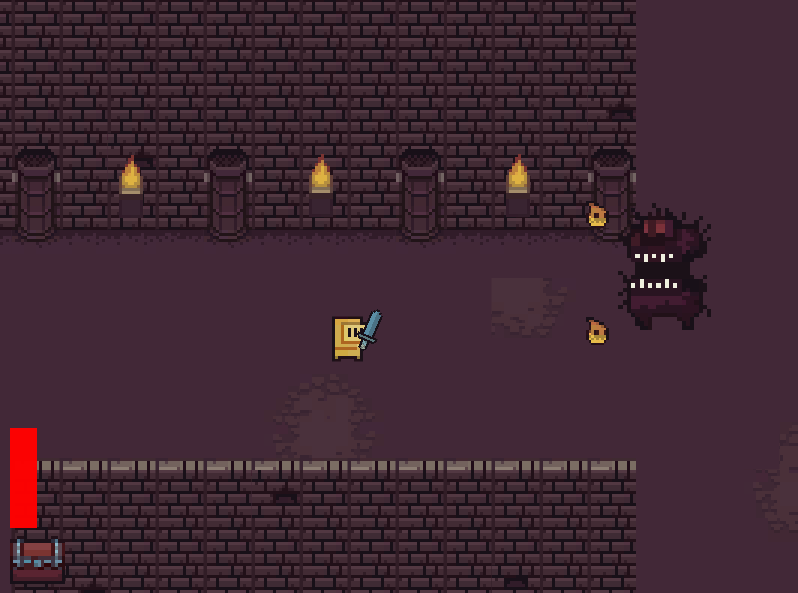
\includegraphics[width = 380px, height=280px]{pictures/boss.png}}\\
\centerline{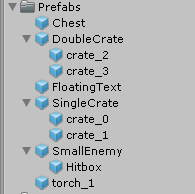
\includegraphics[width = 110px, height=110px]{pictures/prefab.png}}

Но это не значит, что этим ограничиваются игровые механики и ситуации, которые можно реализовать в данном проекте.

\newpage
\section{Вывод}
\Large
В моей курсовой работе была произведена работа с игровым движком Unity, а именно создание 2D игры в жанре Roguelike. В ходе работы был получен опыт работы с самим движком и системой Tilemap для Unity, а также закрепление полученных навыков работы с GitHub, Latex, Beamer.
Болшинство поставленных задач было выполнено.



\newpage
\large
\begin{thebibliography}{100}

\section{Список литературы}
\bibitem{Unity} Основная документация https://docs.unity3d.com/2021.3/Documentation/Manual/WhatsNew2021LTS.html
\bibitem{Unity2} Документация https://learn.unity.com/tutorial/introduction-to-tilemaps
\bibitem{Roguelike} Руководство https://ru.wikipedia.org/wiki/Roguelike
\bibitem{C\#} Microsoft C\# URL: https://docs.microsoft.com/ru-ru/dotnet/csharp/tour-of-csharp/tutorials/
\bibitem{VScode} Visual Studio Code — URL: https://code.visualstudio.com/
\end{thebibliography}

%%%                          %%%
%%%%%%%%%%%%%%%%%%%%%%%%%%%%%%%%

\end{document}